% -----------------------------------------------------------------
% Document class: Article
\documentclass[ a4paper, twoside, 11pt]{article}
\usepackage{../../../macros-general}
\usepackage{../../../macros-article}
% Number of the handout, quiz, exam, etc.
\newcommand{\numero}{01}
\setcounter{numero}{\numero}

% -----------------------------------------------------------------
\begin{document}
\allowdisplaybreaks

\begin{center}
\Large Mec\'anica Vectorial (MECG-1001): Lecci\'on \numero \\[2ex]
\small \textbf{Semestre:} 2017-2018 T\'ermino II \qquad
\textbf{Instructor:} Luis I. Reyes Castro \qquad
\textbf{Paralelo:} 09
\end{center}
\fullskip

% =============================================
\begin{problem}
Para la armadura mostrada en la siguiente figura:
\begin{enumerate}[label=\textbf{\alph*)}]
\item \textbf{3 Puntos:} Encuentre las reacciones el $A$ y $D$. 
\item \textbf{4 Puntos:} Escriba las ocho ecuaciones asociadas con los cuatro nodos de la armadura, denotando compresi\'on con signo positivo y tensi\'on con signo negativo. 
\item \textbf{2 Puntos:} Calcule la fuerza interna en cada eslab\'on. 
\end{enumerate}

\begin{figure}[htb]
\centering
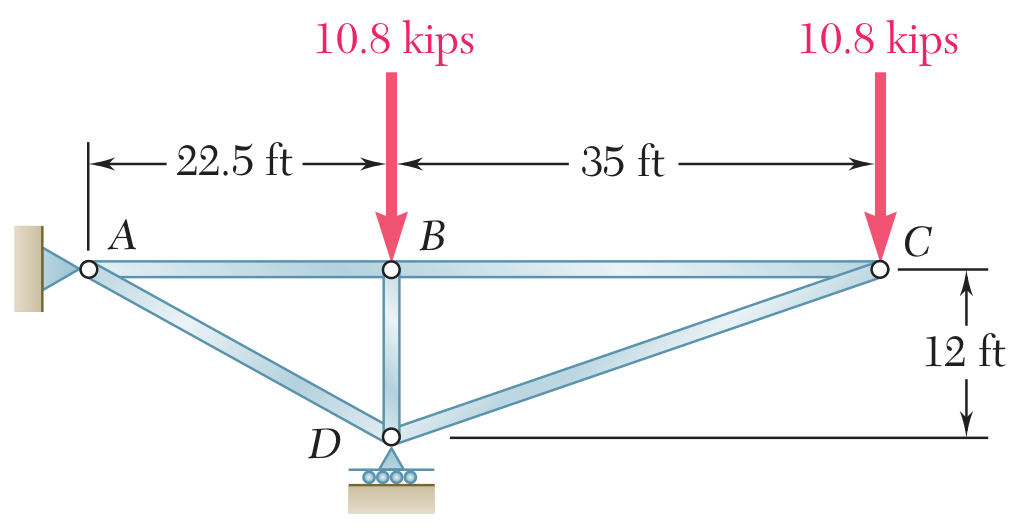
\includegraphics[width=0.56\textwidth]{prob-armadura.jpg}
\end{figure}

\end{problem}
\fullskip

% =============================================
\begin{problem}
Para el armaz\'on mostrado en la siguiente figura:
\begin{enumerate}[label=\textbf{\alph*)}]
\item \textbf{2 Puntos:} Bosqueje los diagramas de cuerpo libre correspondientes. 
\item \textbf{2 Puntos:} Calcule la fuerza que la barra $AFC$ ejerce sobre la barra $BCDE$ en $C$. 
\item \textbf{2 Puntos:} Calcule las reacciones en $A$ y $B$. 
\end{enumerate}

\begin{figure}[htb]
\centering
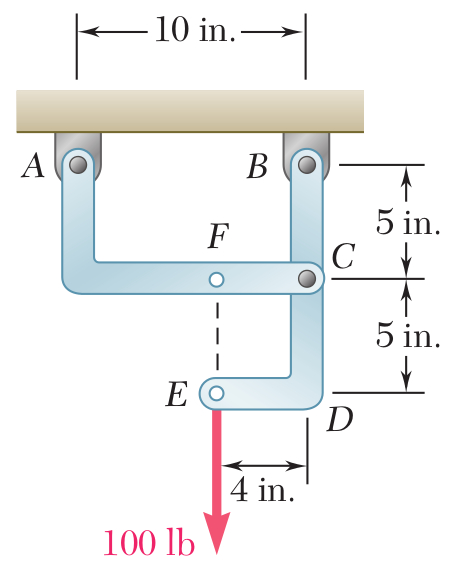
\includegraphics[width=0.28\textwidth]{prob-armazon.jpg}
\end{figure}

\end{problem}
\fullskip

% =============================================
\begin{problem}
\textbf{4 Puntos:} Para la viga mostrada en la siguiente figura encuentre la fuerza cortante $V(x)$ y el momento flector $M(x)$ como funci\'on de la posici\'on $x \in [0,4]$. 

\begin{figure}[htb]
\centering
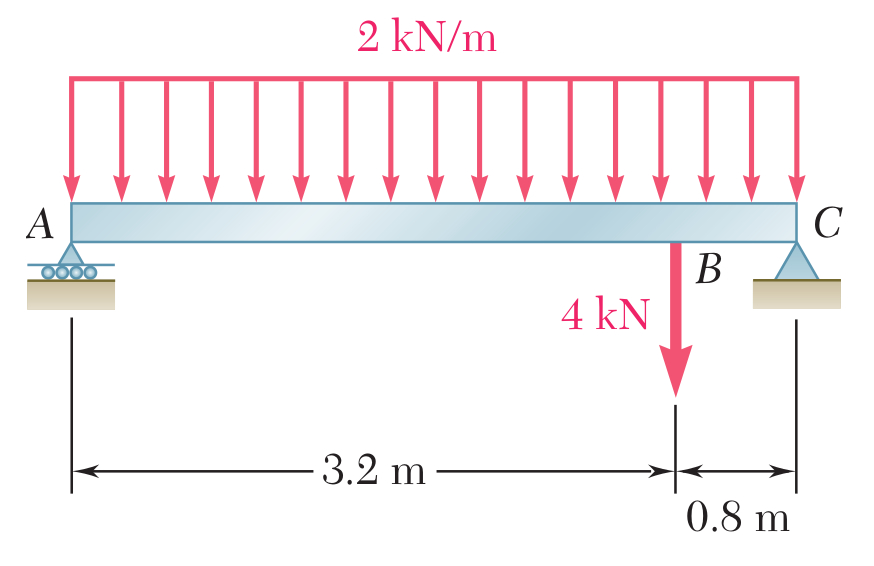
\includegraphics[width=0.42\textwidth]{prob-vigas.jpg}
\end{figure}

\end{problem}
\fullskip

% =============================================
\begin{problem}
El oleoducto mostrado en la siguiente figura est\'a soportado cada 6 ft mediante suspensores verticales fijos a un cable como se muestra en la figura. Debido al peso combinado del ducto y su contenido, cada suspensor experimenta una tensi\'on de 400 lb. Si se sabe que $d_C = 12$ ft, determine: 
\begin{enumerate}[label=\textbf{\alph*)}]
\item \textbf{3 Puntos:} La altura $d_B$. 
\item \textbf{2 Puntos:} Las alturas $d_D$ y $d_E$. 
\item \textbf{2 Puntos:} La tensi\'on m\'axima en el cable. 
\end{enumerate}

\begin{figure}[htb]
\centering
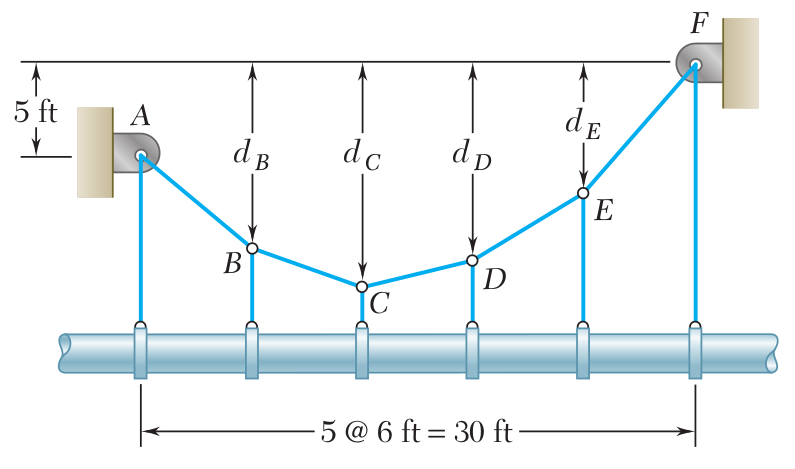
\includegraphics[width=0.52\textwidth]{prob-cables.jpg}
\end{figure}

\end{problem}
\fullskip

\end{document}